% !TEX TS-program = xelatex
% !TEX encoding = UTF-8 Unicode

% Tennessee Technological University
% ME4140 - Fall 2016 - Fall 2017 - ? - Fall 2019 - Fall 2020
% Tristan Hill - September 10, 2020
% Turtorial 2 - Install ROS

\documentclass[12pt]{article}
%\usepackage{/home/thill/Documents/lectures/ros_workshop/ros_tutorial}
\usepackage{/mnt/c/Users/thill/Documents/courses/ros_workshop/ros_tutorial}

% Title and Misc
\newcommand{\MNUM}{2} %Module Number
\newcommand{\MNAME}{Install ROS} %Module Name
\pagestyle{myheadings}
\markright{{\large ME4140 - ROS Workshop - Fall 2021}}

\textwidth=7.0in
\topmargin=-0.6in
\leftmargin=0.5in
\textheight=9.25in
\hoffset=-0.5in
\footskip=0.2in

\begin{document}

\thispagestyle{plain}

\begin{center}
   {\bf \Large ROS Workshop - Tutorial\hspc\MNUM\hspc - \MNAME}\vspace{3mm}\\
   {\bf \large ME 4140 - Introduction to Robotics - Fall 2021} \vspace{5mm}\\
\end{center}

\begin{description}

\item[\textbf{\underline{Overview:}}] \hfill \vspace{3mm}\\
After completing {\it Tutorial 1 - Virtualize Ubuntu}, your new operating system is running, and you are ready to install ROS. You can read more about the installation \href{http://wiki.ros.org/melodic/Installation/Ubuntu}{here} on the wiki.

\item[\textbf{\underline{System Requirements:}}] \hfill \vspace{0mm}

\begin{itemize}
	\item {\bf OS}: This tutorial is intended for the Ubuntu 18.04 LTS operating system. Alternate flavors of 18.04 (i.e. - Mint, Mate, kbuntu) may work but have not been tested.
	\item {\bf Internet:} Your computer must be connected to the internet to proceed. Downloading and installing ROS may take approximately 15 to 30 minutes .


\end{itemize}

\item[\textbf{\underline{Disclaimer:}}] \hfill \vspace{0mm}

\begin{itemize}
	\item {\bf Copy and Paste Errors:}  It is strongly recommended to use copy and paste to enter the commands in this tutorial, but {\RD this will not work correctly in the ilearn PDF viewer}. Use the tutorial webpage or download the PDF to copy the commands directly.

	\item {\bf Backup: } If you are using a virtual machine, it is recommend to make a snaphot of your virtual machine in case you want to revert. (See {\it Tutorial 1 - Virtualize Ubuntu }) 
\end{itemize}

\item[\textbf{\underline{Installation Instructions:}}] \hfill \vspace{0mm}

Press \CTRLKey+\ALTKey+\TKey to open a new terminal, then carefully copy each command and paste it into the terminal then press \ENTERKey. { \bf The terminal commands are shown in gray boxes.}


\begin{enumerate}
	
	
	\item  Setup your sources.list to accept software from packages.ros.org.

	\begin{minted}{text}
sudo sh -c 'echo "deb http://packages.ros.org/ros/ubuntu $(lsb_release 
-sc) main" > /etc/apt/sources.list.d/ros-latest.list'
	\end{minted}
	
	\item Set up your keys which are used authenticate software packages for security.
	
	\begin{minted}[]{text}
sudo apt install curl # if you haven't already installed curl
curl -s https://raw.githubusercontent.com/ros/rosdistro/master/ros.asc 
| sudo apt-key add -
	\end{minted}
	
%	\begin{minted}[]{text}
%sudo apt-key adv --keyserver 'hkp://keyserver.ubuntu.com:80' \ 
%--recv-key C1CF6E31E6BADE8868B172B4F42ED6FBAB17C654
%	\end{minted}
				
	\item Update your Ubuntu system. It is a good idea to do this before installing new packages. 
	
	\begin{minted}[]{text}
sudo apt update
	\end{minted}

\newpage
	
	\item Download and install ROS Melodic Desktop-Full. Depending on your network connection this step will take some time. Now is a good time to get a \Coffeecup \Cooley.  
	
	\begin{minted}[]{text}
sudo apt install ros-melodic-desktop-full
	\end{minted}

\item Evironment Setup (2 separate commands). This appends the {\it .bashrc} file which runs each time you open a new terminal. 
\begin{minted}{text} 
echo "source /opt/ros/melodic/setup.bash" >> ~/.bashrc
\end{minted}

\begin{minted}{text} 
source ~/.bashrc 
\end{minted}

\item Install Development Tools. You are almost there! 
\begin{minted}{text} 
sudo apt install python-rosdep python-rosinstall \ 
python-rosinstall-generator python-wstool build-essential
\end{minted}

	\item Initialize rosdep (2 separate commands) 
	\begin{minted}[]{text}
sudo rosdep init
	\end{minted}
	
	\begin{minted}[]{text} 
rosdep update
	\end{minted}


		


After completing Step 7 you have installed ROS on your Ubuntu system. Now it is time to test the installation. 
\end{enumerate}

\newpage

\item[\textbf{\underline{Test ROS Installation}}]

\item Close all open terminal windows. Next, open a new terminal and try the following command.\\
\begin{minted}{text}  
roscore
\end{minted}

If the installation was successful, the terminal output will be {\it similar} to the image below. \vspace{3mm}\\

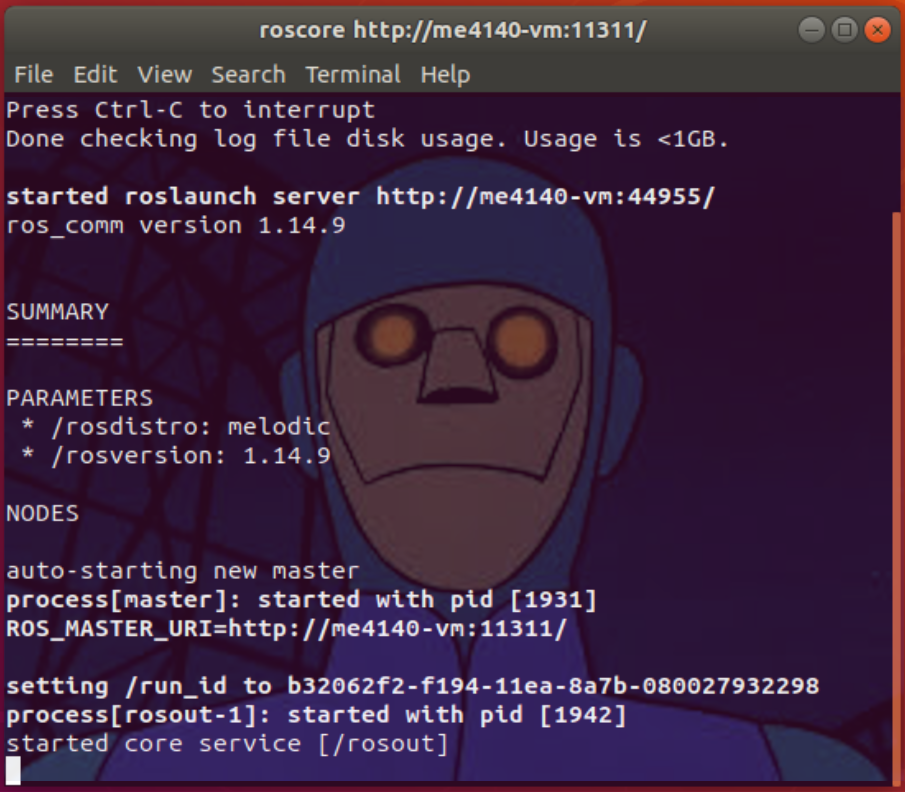
\includegraphics[scale=1]{roscore_charlie.png} \vspace{2mm}\\

Abort the roscore process by clicking in the terminal and pressing \CTRLKey + \CKey, then close the terminal window. Congratulations, you have installed ROS Melodic.

\item[\textbf{\underline{Tutorial Complete:}}] \hfill \vspace{3mm}\\

If you see ROS start in the terminal your ROS installation was successful!


\end{description}
\end{document}
